% Created 2025-07-04 Fri 17:21
\documentclass[10pt]{article}
\usepackage{graphicx}
\usepackage{longtable}
\usepackage{wrapfig}
\usepackage{rotating}
\usepackage[normalem]{ulem}
\usepackage{amsmath}
\usepackage{amssymb}
\usepackage{capt-of}
\usepackage{hyperref}
\usepackage[newfloat]{minted}
\usepackage[a4paper, total={6.5in, 9in}]{geometry}
\usepackage{minted}
\setminted{breaklines}
\usepackage[utf8]{inputenc}
\renewcommand{\familydefault}{\sfdefault}
\usemintedstyle{vs}
\usepackage[most]{tcolorbox}
\usepackage{CJKutf8}
\usepackage{xurl}
\usepackage{fontawesome5}
\usepackage{hyperref}
\usepackage{graphicx}
\usepackage{float}
\author{Vincent Conus\thanks{vincent.conus@protonmail.com}}
\date{2023-12-22}
\title{KRIA board Ubuntu LTS 22.04 Install}
\hypersetup{
 pdfauthor={Vincent Conus},
 pdftitle={KRIA board Ubuntu LTS 22.04 Install},
 pdfkeywords={},
 pdfsubject={A separated export for the Ubuntu install process},
 pdfcreator={Emacs 30.1 (Org mode 9.7.11)}, 
 pdflang={English}}
\begin{document}

\maketitle
\tableofcontents

\section{Preparing and booting a Ubuntu 22.04 media}
\label{sec:orgde4e43f}
An \href{https://ubuntu.com/download/amd-xilinx}{official Ubuntu image} exists and is
provided by Xilinx, allowing the OS installation to be quick and
straightforward.
Ubuntu is a common and easy to use distribution. Furthermore,
it allows to install ROS2 as a package, which is most convenient and will be
done later in this guide.

Once the image has been downloaded at \href{https://ubuntu.com/download/amd-xilinx}{Canonical's page}
we can flash it onto the SD card, with the following instructions.

\begin{tcolorbox}[colback=red!5!white,colframe=red!75!black]
\textbf{DANGER}: The next part involve the \texttt{dd} command writing on disks!!!
As always with the dd command, thou have to be \textbf{VERY} careful on what arguments
thou give. Selecting the wrong disk will result on the destruction of
thy data !!
\uline{If you are unsure of what to do, seek assistance !}
\end{tcolorbox}

With the image available on thy machine and a SD card visible as \texttt{/dev/sda} device\footnote{Again, it is \uline{critical} to be 100$\backslash$% certain that you are working with
the correct device!}
one can simply run the \texttt{dd} command as follow to write the image to a previously formatted drive (here \texttt{/dev/sda}):

\begin{minted}[frame=single,framesep=2mm,baselinestretch=1.2,linenos,breaklines,fontsize=\footnotesize]{sh}
unxz iot-limerick-kria-classic-desktop-2204-20240304-165.img.xz
sudo dd if=iot-limerick-kria-classic-desktop-2204-20240304-165.img \
     of=/dev/sda status=progress bs=8M && sync
\end{minted}


Once the SD card is flashed and put back in the board, the micro-USB cable can be
connected from the PC to the board. It is then possible to
connect to the board in serial with an appropriate tool, for example \texttt{picocom},
as in the following example (the serial port that "appeared" was the \texttt{/dev/ttyUSB1} in this case\footnote{If two boards are plugged in for serial, the second one will be \texttt{/dev/ttyUSB5}, then \texttt{USB9} and so on.},
and the 115200 bit-rate is the default value for the board):

\begin{minted}[frame=single,framesep=2mm,baselinestretch=1.2,linenos,breaklines,fontsize=\footnotesize]{sh}
sudo picocom /dev/ttyUSB1 -b 115200
\end{minted}

In my case, I am using Emacs's \texttt{serial-term}:
\begin{minted}[frame=single,framesep=2mm,baselinestretch=1.2,linenos,breaklines,fontsize=\footnotesize]{sh}
M-x serial-term RET /dev/ttyUSB1 RET 115200 RET
\end{minted}

The default username / password pair for the very first boot is \texttt{ubuntu} and \texttt{ubuntu}. You will then be prompted to enter a new password.

Once logged in, it is typically easier and more convenient to connect the board
using SSH. When the board is connected to the network, it is possible to know
it's IP address with the \texttt{IP} command; then it is possible to connect to
the board with ssh, as follow (example, with the first command to be run on the board
and the second one on the host PC, both without the first placeholder hostnames):
\begin{minted}[frame=single,framesep=2mm,baselinestretch=1.2,linenos,breaklines,fontsize=\footnotesize]{sh}
kria# ip addr

host# ssh ubuntu@192.168.4.11
\end{minted}
\section{Network and admin setups}
\label{sec:org8ce2ad4}
This section presents a variety of extra convenience configurations
that can be used when setting-up the Kria board.
\subsection{Static IP address}
\label{sec:org5b9b9fd}
A static IP can be set by writing the following
configuration into your \texttt{netplan} configuration file\footnote{The \texttt{chmod} command is used to update the permissions and silence some warnings}.

The name of the files might vary:
\begin{minted}[frame=single,framesep=2mm,baselinestretch=1.2,linenos,breaklines,fontsize=\footnotesize]{sh}
sudo chmod 0600 /etc/netplan/50-cloud-init.yaml 
sudo nano /etc/netplan/50-cloud-init.yaml
\end{minted}

You can then set the wanted IP as follow\footnote{For the routing part, it is key to have the \texttt{to} with a \texttt{'-'} in front of
it; and then the \texttt{via} without, but aligned with the \texttt{t}.}:
\begin{minted}[frame=single,framesep=2mm,baselinestretch=1.2,linenos,breaklines,fontsize=\footnotesize]{yaml}
network:
  renderer: NetworkManager
  version: 2
  ethernets:
    eth0:
      dhcp4: false
      addresses:
        - 192.168.11.107/24
      routes:
        - to: default
          via: 192.168.11.1
      nameservers:
        addresses: [192.168.11.1]
\end{minted}

Finally, the change in settings can be applied
as follow:

\begin{minted}[frame=single,framesep=2mm,baselinestretch=1.2,linenos,breaklines,fontsize=\footnotesize]{sh}
sudo netplan apply
\end{minted}
\subsection{{[}facultative] Proxy for \texttt{apt} on Nagoya University network}
\label{sec:orge1b3da8}
This is a configuration specific to use the board at Nagoya University, on the
local network. The following configuration is to be used in \texttt{/etc/apt/apt.conf}:
\begin{minted}[frame=single,framesep=2mm,baselinestretch=1.2,linenos,breaklines,fontsize=\footnotesize]{bash}
Acquire::http::Proxy "http://172.24.8.1:8080";
Acquire::https::Proxy "http://172.24.8.1:8080";
\end{minted}
\subsection{{[}facultative] Check the system clock}
\label{sec:org9f81a9a}

\subsection{{[}facultative] \texttt{root} password}
\label{sec:orgab3d827}
\begin{tcolorbox}[colback=orange!5!white,colframe=orange!75!black]
\textbf{WARNING}: Depending on your use-case, the setup presented in this
subsection can be a critical security breach as it remove the need for a root
password to access the admin functions of the board's Linux.
\uline{When in doubt, do not apply this configuration!!}
\end{tcolorbox}

If you board does not hold important data
and is available to you only, for test or development,
it might be convenient for the \texttt{sudo} tool to not ask for the
password all the time.
This change can be done by editing the sudoers file, and
adding the parameter \texttt{NOPASSWD}
at the \texttt{sudo} line:

\begin{minted}[frame=single,framesep=2mm,baselinestretch=1.2,linenos,breaklines,fontsize=\footnotesize]{sh}
sudo visudo

%sudo   ALL=(ALL:ALL) NOPASSWD: ALL
\end{minted}

Again, this is merely a convenience setup for devices staying at you desk. If
the board is meant to be used in any kind of production setup, a password
should be set for making administration tasks.

With all of these settings, you should be able to update the software of your
board without any issues:
\begin{minted}[frame=single,framesep=2mm,baselinestretch=1.2,linenos,breaklines,fontsize=\footnotesize]{sh}
sudo apt update
sudo apt dist-upgrade
sudo reboot now
\end{minted}
\subsection{Adding Xilinx specific repositories}
\label{sec:orgb7b07e5}
The following commands will add \texttt{PPA} repositories that are specific for Xilinx boards using Ubuntu.
It is then possible to update the package list and eventually upgrade to some new packages.
\begin{minted}[frame=single,framesep=2mm,baselinestretch=1.2,linenos,breaklines,fontsize=\footnotesize]{sh}
sudo add-apt-repository ppa:ubuntu-xilinx/updates
sudo add-apt-repository ppa:xilinx-apps/ppa
sudo apt update
sudo apt upgrade
\end{minted}
\subsection{{[}facultative] Installing Docker}
\label{sec:orgd902ed7}
It is possible to have a version of Docker installed simply by using the available repository,
but since we are on Ubuntu, a PPA is available from Docker in order to have the most up-to-date version.

Following \href{https://docs.docker.com/engine/install/ubuntu/\#install-using-the-repository}{the official documentation}, the following steps can be taken to install the latest version of
Docker on a Ubuntu system. The last command is meant to test the install.
If everything went smoothly, you should see something similar to what is presented
in the figure \ref{fig:org268f2b0} below, after the commands:

\begin{minted}[frame=single,framesep=2mm,baselinestretch=1.2,linenos,breaklines,fontsize=\footnotesize]{sh}
sudo apt-get update
sudo apt-get install ca-certificates curl
sudo install -m 0755 -d /etc/apt/keyrings
curl -fsSL https://download.docker.com/linux/ubuntu/gpg | \
    sudo gpg --dearmor -o /etc/apt/keyrings/docker.gpg

sudo chmod a+r /etc/apt/keyrings/docker.gpg

echo \
    "deb [arch="$(dpkg --print-architecture)" \
  signed-by=/etc/apt/keyrings/docker.gpg] \
  https://download.docker.com/linux/ubuntu \
  "$(. /etc/os-release && \
         echo "$VERSION_CODENAME")" stable" | \
    sudo tee /etc/apt/sources.list.d/docker.list > /dev/null

sudo apt-get update
sudo apt-get install docker-ce docker-ce-cli \
     containerd.io docker-buildx-plugin docker-compose-plugin
sudo usermod -aG docker $USER
newgrp docker

docker run hello-world
\end{minted}

\begin{figure}[htbp]
\centering
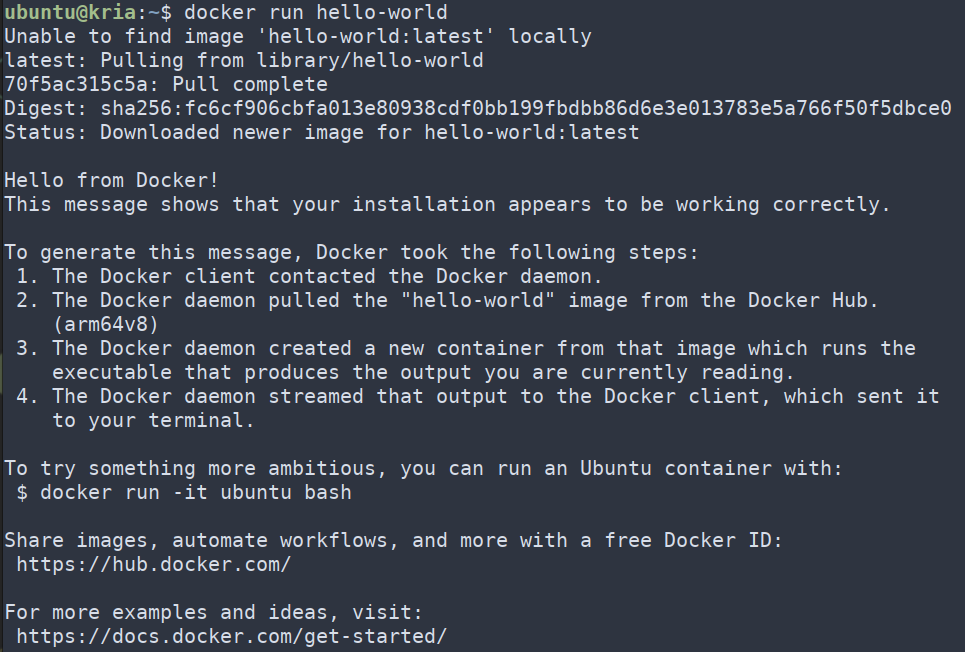
\includegraphics[width=.7\textwidth]{img/hello-docker.png}
\caption{\label{fig:org268f2b0}The return of a successful run of the \texttt{hello world} test Docker container.}
\end{figure}
\subsection{{[}recommended] Purging \texttt{snap}}
\label{sec:org52e1bee}
As the desktop-specific software are not used at all in the case
of our project, there are some packages that can be purges in order for the
system to become more lightweight.

In particular, the main issue with Ubuntu systems is the forced integration of
Snap packages. Here are the command to use in order to remove all of that.
These steps take a lot of time and need to be executed in that specific order\footnote{The \texttt{snap} packages depends on each others. Dependencies
cannot be remove before the package(s) that depends on them,
thus the specific delete order.},
but the system fan runs sensibly slower without all of this stuff.

Note that this all process is rather slow and can take up to 30min to complete.
\begin{minted}[frame=single,framesep=2mm,baselinestretch=1.2,linenos,breaklines,fontsize=\footnotesize]{sh}
sudo systemctl disable snapd.service
sudo systemctl disable snapd.socket
sudo systemctl disable snapd.seeded.service

sudo snap list #show installed package, remove them all:
sudo snap remove --purge firefox
sudo snap remove --purge gnome-3-38-2004
sudo snap remove --purge gnome-42-2204
sudo snap remove --purge gtk-common-themes
sudo snap remove --purge snapd-desktop-integration
sudo snap remove --purge snap-store
sudo snap remove --purge bare
sudo snap remove --purge core20
sudo snap remove --purge core22
sudo snap remove --purge snapd
sudo snap list # check that everything is uninstalled

sudo rm -rf /var/cache/snapd/
sudo rm -rf ~/snap
sudo apt autoremove --purge snapd

# check once more that there is no more snap on the system
systemctl list-units | grep snapd 
\end{minted}
\subsection{{[}facultative] Other unused heavy packages}
\label{sec:orgaba5db9}
Some other pieces of software can safely be removed since the desktop is
not to be used.
\begin{minted}[frame=single,framesep=2mm,baselinestretch=1.2,linenos,breaklines,fontsize=\footnotesize]{sh}
sudo apt-get autoremove --purge yaru-theme-icon \
     fonts-noto-cjk yaru-theme-gtk vim-runtime \
     ubuntu-wallpapers-jammy humanity-icon-theme

sudo apt-get autoclean
sudo reboot now
\end{minted}
\subsection{{[}facultative] Slow boot services to disable}
\label{sec:orga8fafcb}
These packages (in particular the first one) are taking up a LOT of time at boot while providing no benefits\footnote{The CUPS and Docker services will be activated when used instead of during boot time.}.

It is possible to disable them as follow:
\begin{minted}[frame=single,framesep=2mm,baselinestretch=1.2,linenos,breaklines,fontsize=\footnotesize]{sh}
sudo systemctl disable systemd-networkd-wait-online.service
sudo systemctl disable NetworkManager-wait-online.service
sudo systemctl disable cups.service
sudo systemctl disable docker.service
sudo systemctl disable containerd.service
sudo systemctl disable cloud-init-local.service
\end{minted}

Additional, potentially unused services can be found using the very handy command:
\begin{minted}[frame=single,framesep=2mm,baselinestretch=1.2,linenos,breaklines,fontsize=\footnotesize]{sh}
sudo systemd-analyze blame
\end{minted}
\subsection{{[}facultative] Adding a swap partition}
\label{sec:org80afbe9}
This part is very optional, in particular as it might slow down a bit the
boot time of the board (\textasciitilde{}2s), however it might become handy to have swap memory
available to avoid system failure under heavy use.

This whole procedure must be done externally, with the board system SD card
mounted on a host PC as an external volume.  As it is highly platform dependant,
I will not give a detailed explanation on how to do it, yet here are the key
points that should be done:
\begin{itemize}
\item Shutdown the Kria board, take out the SD card and put it in a host machine.
\item Make sure the disk is visible.
\item Make sure all volumes are \textbf{unmounted}.
\item Resize the main \texttt{root} partition (\textbf{not} the \texttt{boot}) so a space the size of the
wanted swap is free \textbf{after} the partition. You'd want something around 1GB.
\item In the empty space, create a new partition, which type is "linux swap".
\item Find and take note of the UUID of the new partition. This is useful hereafter.
\item \texttt{sync}
\item Un-mount everything, eject SD card.
\item Put the SD card back in the Kria.
\item Boot back to Ubuntu.
\end{itemize}

Going back on the Kria board Ubuntu after boot, the \texttt{/etc/fstab} file can be
updated as follow, modulo your actual UUID for the newly created partition, to
enable swap at boot time.
\begin{minted}[frame=single,framesep=2mm,baselinestretch=1.2,linenos,breaklines,fontsize=\footnotesize]{sh}
sudo -s
echo "UUID=8b13ed05-a91d-4x50-a44a-e654a0c67a2c none   swap    sw      0       0" >> /etc/fstab
reboot now
\end{minted}
\subsection{{[}OLD] Enabling \texttt{remoteproc} with Device-Tree patching}
\label{sec:orged5b1fd}
One of the advantage of this Kria board, as cited previously, is the presence of
multiple types of core (APU, MCU, FPGA) on the same chip.

The part in focus in this guide is the usage of both the APU, running
a Linux distribution and ROS2; and the MCU, running FreeRTOS and micro-ROS.
Online available guides\footnote{A \href{https://speakerdeck.com/fixstars/fpga-seminar-12-fixstars-corporation-20220727}{slideshow} (JP) from Fixstar employees presents how to use the device
tree to enable the communication between the cores.} \textsuperscript{,}\,\footnote{A \href{https://zenn.dev/ryuz88/articles/kv260\_setup\_memo\_ubuntu22 }{blog post} (JP) shows all major steps on how to enable the \texttt{remoteproc}.} also provide information on how to deploy these types
of systems and enabling \texttt{remoteproc} for the Kria board, but this guide
will show a step-by-step, tried process to have a heterogeneous system
up and running.

The communication between both side is meant to be done using shared memory, but
some extra setup is required in order to be running the real-time firmware, in particular
for deploying micro-ROS on it.

As a first step in that direction, this section of the report
will present how to setup and use as an example firmware that utilizes the
\texttt{remoteproc} device in Linux in order to access shared memory
and communicate with the real-time firmware using the RPMsg system.

The communication system and interaction from the Linux side towards the real-time capable core
is not enabled by default within the Ubuntu image provided by Xilinx.

In that regard, some modification of the device tree overlay (DTO) is required in order to have
the \texttt{remoteproc} system starting.
\subsubsection{Patching the device tree for RPMsg (standard, kernel space mode)}
\label{sec:orgcc03c02}
Firstly, we need to get the original firmware device tree, converted
into a readable format (DTS):

\begin{minted}[frame=single,framesep=2mm,baselinestretch=1.2,linenos,breaklines,fontsize=\footnotesize]{sh}
sudo dtc /sys/firmware/fdt 2> /dev/null > system.dts
\end{minted}

Then, a custom-made patch file can be downloaded and applied.
This file is available at the URL visible in the command below.

\begin{minted}[frame=single,framesep=2mm,baselinestretch=1.2,linenos,breaklines,fontsize=\footnotesize]{sh}
wget https://gitlab.com/sunoc/xilinx-kria-kv260-documentation/-/raw/main/src/system.patch

patch system.dts < system.patch
\end{minted}
\subsubsection{Kernel \texttt{cmd} edit}
\label{sec:org6ba9ce7}
As for the board to be able to reserve the correct amount of memory with the new settings, some
\texttt{cma} kernel configuration is needed\footnote{The overlapping memory will not prevent the board to boot,
but it disables the PWM for the CPU fan, which will then run at full speed, making noise.}:

\begin{minted}[frame=single,framesep=2mm,baselinestretch=1.2,linenos,breaklines,fontsize=\footnotesize]{sh}
sudo nano /etc/default/flash-kernel

LINUX_KERNEL_CMDLINE="quiet splash cma=512M cpuidle.off=1"
LINUX_KERNEL_CMDLINE_DEFAULTS=""
sudo flash-kernel
\end{minted}

Now the DTS file has been modified, one can regenerate the binary and place it on the \texttt{/boot} partition
and reboot the board:

\begin{minted}[frame=single,framesep=2mm,baselinestretch=1.2,linenos,breaklines,fontsize=\footnotesize]{sh}
dtc -I dts -O dtb system.dts -o user-override.dtb
sudo mv user-override.dtb /boot/firmware/
sudo reboot now
\end{minted}
\subsubsection{Checking the patching}
\label{sec:orgf4943fa}
After rebooting, you can check the content of the \verb|remoteproc| system directory,
and a \texttt{remoteproc0} device should be visible, as follow:

\begin{minted}[frame=single,framesep=2mm,baselinestretch=1.2,linenos,breaklines,fontsize=\footnotesize]{sh}
ls /sys/class/remoteproc/
#  remoteproc0
\end{minted}

If it is the case, it means that the patch was successful and  that the remote processor is
ready to be used!
\pagebreak
\subsection{{[}NEW] Enabling \texttt{remoteproc} for RPMsg in userspace with device-tree patch}
\label{sec:org09c0173}
\subsubsection{Kernel \texttt{cmd} edit}
\label{sec:orge6c4095}
\begin{minted}[frame=single,framesep=2mm,baselinestretch=1.2,linenos,breaklines,fontsize=\footnotesize]{sh}
sudo nano /etc/default/flash-kernel

LINUX_KERNEL_CMDLINE="quiet splash cma=512M cpuidle.off=1"
LINUX_KERNEL_CMDLINE_DEFAULTS=""
sudo flash-kernel
\end{minted}
\subsubsection{Patching the device tree for RPMsg in userspace}
\label{sec:org482c6bd}
The  \texttt{system\_uio.patch}
\begin{minted}[frame=single,framesep=2mm,baselinestretch=1.2,linenos,breaklines,fontsize=\footnotesize]{bash}
sudo dtc /sys/firmware/fdt 2> /dev/null > system.dts

wget https://gitlab.com/sunoc/xilinx-kria-kv260-documentation/-/raw/main/src/system_uio.patch

patch system.dts < system_uio.patch

dtc -I dts -O dtb system.dts -o user-override.dtb
sudo mv user-override.dtb /boot/firmware/
sudo reboot now
\end{minted}
\subsubsection{Checking the patching}
\label{sec:org4a21a44}
If everything went correctly, on reboot and re-logging in the device, you should
see an output to the following command:
\begin{minted}[frame=single,framesep=2mm,baselinestretch=1.2,linenos,breaklines,fontsize=\footnotesize]{bash}
ls /sys/class/remoteproc/
\end{minted}
\subsection{{[}NEW] Nagoya University proxy and NTP}
\label{sec:org11d7686}
\begin{tcolorbox}[colback=orange!5!white,colframe=orange!75!black]
\textbf{WARNING}: This setup is needed when using the KRIA board with wired internet
at Honda Lab in Nagoya University, because of the local network proxy.
\end{tcolorbox}

Two main addresses for working behind the lab's local network proxy are:
\begin{itemize}
\item \texttt{172.24.8.1} for HTTP and HTTPS proxy.
\item \texttt{172.24.8.19} for the local NTP server.
\end{itemize}

The following sub-sections will present how to use these.
\subsubsection{General HTTP proxy}
\label{sec:org9ba84df}
These lines must be places at the end of the \texttt{\textasciitilde{}/.bashrc} file:
\begin{minted}[frame=single,framesep=2mm,baselinestretch=1.2,linenos,breaklines,fontsize=\footnotesize]{bash}
export http_proxy="172.24.8.1:8080"
export https_proxy="172.24.8.1:8080"
export no_proxy="localhost,127.0.0.1,::1"
\end{minted}
\subsubsection{HTTP proxy for the package manager}
\label{sec:orgc37acaa}
These lines must be places at the end of the \texttt{/etc/apt/apt.conf} file:
\begin{minted}[frame=single,framesep=2mm,baselinestretch=1.2,linenos,breaklines,fontsize=\footnotesize]{text}
Acquire::http::Proxy "http://172.24.8.1:8080";
Acquire::https::Proxy "http://172.24.8.1:8080";
\end{minted}
\subsubsection{Local NTP server}
\label{sec:org1829eaf}
Installing a NTP tool:
\begin{minted}[frame=single,framesep=2mm,baselinestretch=1.2,linenos,breaklines,fontsize=\footnotesize]{bash}
sudo apt update
sudo apt install systemd-timesyncd
\end{minted}

These lines must be places at the end of the \texttt{/etc/systemd/timesyncd.conf} file:
\begin{minted}[frame=single,framesep=2mm,baselinestretch=1.2,linenos,breaklines,fontsize=\footnotesize]{text}
[Time]
NTP=172.24.8.19
\end{minted}

Start and enable the NTP tool systemd daemon:
\begin{minted}[frame=single,framesep=2mm,baselinestretch=1.2,linenos,breaklines,fontsize=\footnotesize]{bash}
sudo systemctl start systemd-timesyncd
sudo systemctl enable systemd-timesyncd
timedatectl
\end{minted}
\subsubsection{Git forges SSH access through proxy}
\label{sec:org1948c67}
A SSH through HTTP tunneling tool must be installed:
\begin{minted}[frame=single,framesep=2mm,baselinestretch=1.2,linenos,breaklines,fontsize=\footnotesize]{bash}
sudo apt update
sudo apt install corkscrew
\end{minted}

These lines must be places at the end of the \texttt{\textasciitilde{}/.gitconfig} file:
\begin{minted}[frame=single,framesep=2mm,baselinestretch=1.2,linenos,breaklines,fontsize=\footnotesize]{text}
Host github.com
     User git
     Port 443
     Hostname ssh.github.com
     TCPKeepAlive yes
     IdentityFile ~/.ssh/id_ed25519
     IdentitiesOnly yes
     ProxyCommand /usr/bin/corkscrew 172.24.8.1 8080 %h %p

Host gitlab.com
     User git
     Port 443
     Hostname altssh.gitlab.com
     IdentityFile ~/.ssh/id_ed25519
     ProxyCommand /usr/bin/corkscrew 172.24.8.1 8080 %h %p
\end{minted}
\subsection{{[}DEPRECATED] Nanzan Net Proxy and DNS}
\label{sec:org1aeecbc}
\begin{tcolorbox}[colback=orange!5!white,colframe=orange!75!black]
\textbf{WARNING}: This setup is not needed anymore when using Honda-sensei's lab
wired network.
Adding it will cause the DNS to FAIL!
This section is kept as a reference.
\end{tcolorbox}
An issue that can occur when connecting the board to the internet is the
conflicting situation with the university proxy.
Indeed, as the network at Nanzan University requires to go through a proxy,
some DNS errors appeared.

In that case, it might become needed to setup the proxy for the school.

This can be done as follow, by exporting a https base proxy configuration
containing you AXIA credentials (this is specific to Nanzan University IT system),
then by consolidating the configuration for other types of connections in the \texttt{bashrc}:

\begin{minted}[frame=single,framesep=2mm,baselinestretch=1.2,linenos,breaklines,fontsize=\footnotesize]{sh}
export https_proxy="http://<AXIA_username>:\
       <AXIA_psw>@proxy.ic.nanzan-u.ac.jp:8080"

echo "export http_proxy=\""$https_proxy"\"" >> ~/.bashrc
echo "export https_proxy=\""$https_proxy"\"" >> ~/.bashrc
echo "export ftp_proxy=\""$https_proxy"\"" >> ~/.bashrc
echo "export no_proxy=\"localhost, 127.0.0.1,::1\"" >> ~/.bashrc
\end{minted}

Eventually the board can be rebooted in order for the setup to get applied cleanly.
\subsection{{[}DEPRECATED] Jupyter notebook setup}
\label{sec:orgf45f1a4}
Here are some instruction on how to install and setup Jupyter on a KRIA board,
accessing it remotely and using it for making data analysis.

The following commands will set the required packages and install Jupyter itself\footnote{Alongside other packages useful for data analysis, such as \texttt{pandas} or \texttt{numpy}.}:
\begin{minted}[frame=single,framesep=2mm,baselinestretch=1.2,linenos,breaklines,fontsize=\footnotesize]{sh}
sudo apt-get update && sudo apt-get install python3 python3-pip python3-venv python3-virtualenv

virtualenv myjupyter
source ./myjupyter/bin/activate
python3 -m pip install jupyter pandas numpy matplotlib scipy

sudo reboot now
\end{minted}

Then in a terminal on your host machine (not on the KRIA board), you can run the following command\footnote{In this example, the full \texttt{username@IP} is used, but a \texttt{.ssh/config} is also usable.} to bind local ports:
\begin{minted}[frame=single,framesep=2mm,baselinestretch=1.2,linenos,breaklines,fontsize=\footnotesize]{sh}
ssh -L 8888:localhost:8888 ubuntu@192.168.11.107
\end{minted}

Then on the opened SSH shell to the KRIA board:
\begin{minted}[frame=single,framesep=2mm,baselinestretch=1.2,linenos,breaklines,fontsize=\footnotesize]{sh}
source ./myjupyter/bin/activate
jupyter notebook
\end{minted}

From there, it is possible to use the displayed URL (something that looks like
\texttt{http://localhost:8888/tree?token}) to access the remote Notebook system from a local web browser.
It is possible to do so with \texttt{localhost} since we have the \texttt{ssh} port map connection going on.

Eventually creating Notebooks and stuff, it is possible to obtain a situation like shown in the figure \ref{fig:orgd6b5788} below.

\begin{figure}[htbp]
\centering
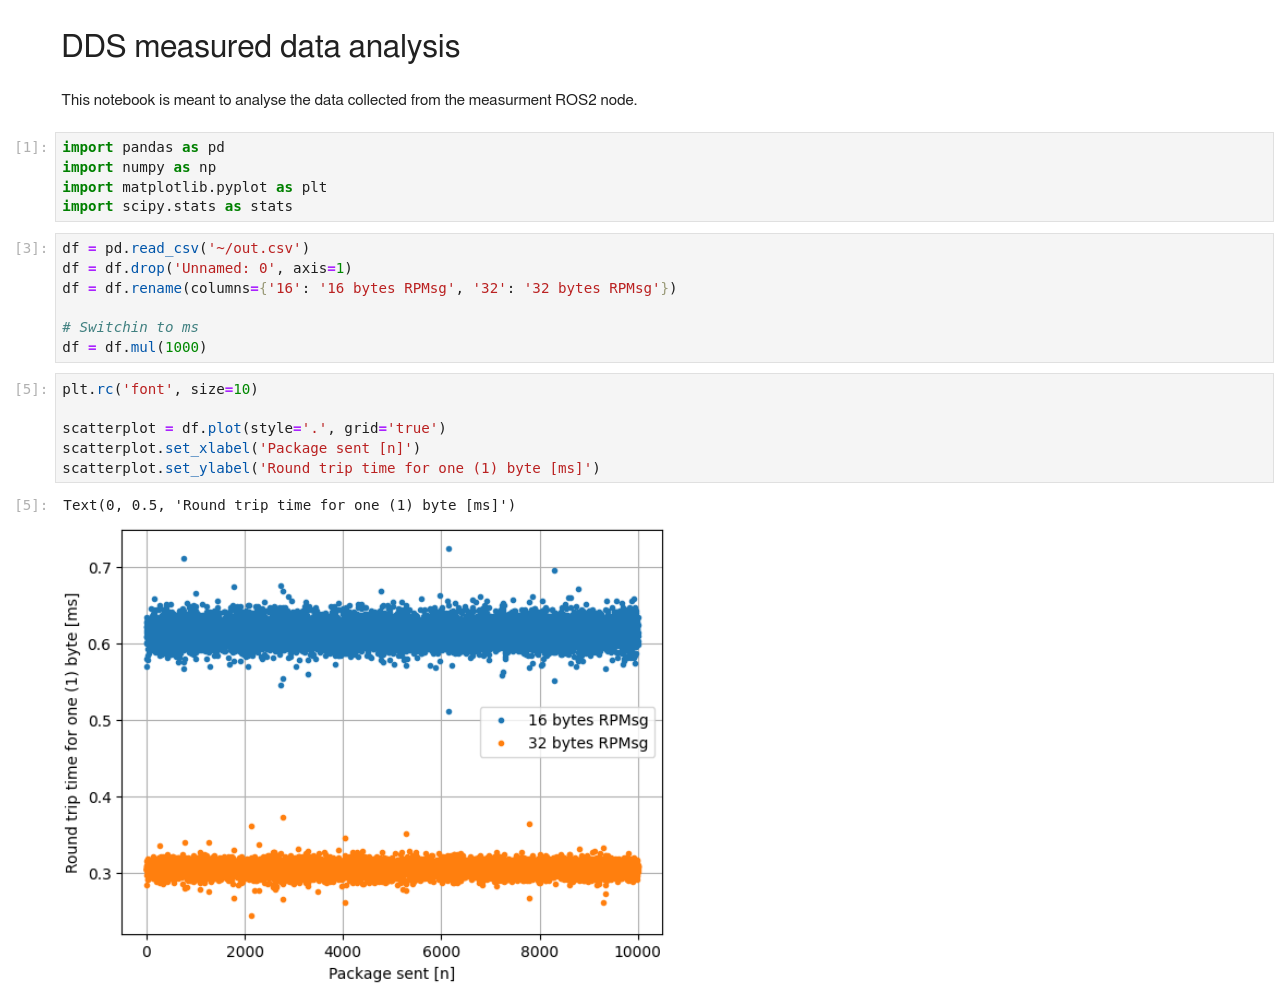
\includegraphics[width=.6\textwidth]{img/jupyter.png}
\caption{\label{fig:orgd6b5788}A test Jupyter Notebook for CSV data analysis.}
\end{figure}
\subsection{{[}TODO] Using a PetaLinux kernel in Ubuntu}
\label{sec:org3870bbe}
TBD
\section{RPMsg standalone evaluation}
\label{sec:org1434d1b}
\subsection{{[}TODO] RPMsg Cortex R5F demonstration firmware}
\label{sec:orgcfd272e}
\subsection{RPMsg \texttt{echo\_test} software}
\label{sec:orgf4cfd61}
In order to test the deployment of the firmware on the R5F side, and in particular
to test the RPMsg function, we need some program on the Linux side of the KRIA
board to "talk" with the real-time side.

Some source is provided by Xilinx to build a demonstration software that does
this purpose: specifically interact with the demonstration firmware.

Here are the steps required to obtain the sources, and build the program.

As a reminder, this is meant to be done on the Linux running on the
KRIA board, NOT on your host machine !

\begin{minted}[frame=single,framesep=2mm,baselinestretch=1.2,linenos,breaklines,fontsize=\footnotesize]{sh}
git clone https://github.com/Xilinx/meta-openamp.git
cd  meta-openamp
git checkout xlnx-rel-v2022.2
cd  ./recipes-openamp/rpmsg-examples/rpmsg-echo-test
make
sudo ln -s $(pwd)/echo_test /usr/bin/
\end{minted}

Once this is done, it it possible to run the test program from the KRIA board's Ubuntu
by running the \texttt{echo\_test} command.
\end{document}
